\documentclass[a4paper,12pt]{article}
\usepackage{fancyhdr}
\usepackage{fancyheadings}
\usepackage[ngerman,german]{babel}
\usepackage{german}
\usepackage[utf8]{inputenc}
%\usepackage[latin1]{inputenc}
\usepackage[active]{srcltx}
%\usepackage{algorithm}
%\usepackage[noend]{algorithmic}
\usepackage{amsmath}
\usepackage{amssymb}
\usepackage{amsthm}
\usepackage{bbm}
\usepackage{enumerate}
\usepackage{graphicx}
\usepackage{ifthen}
\usepackage{listings}
%\usepackage{struktex}
\usepackage{hyperref}
\usepackage{enumitem}
%\usepackage{wrapfig}

\pagenumbering{gobble}

%%%%%%%%%%%%%%%%%%%%%%%%%%%%%%%%%%%%%%%%%%%%%%%%%%%%%%
%%%%%%%%%%%%%% EDIT THIS PART %%%%%%%%%%%%%%%%%%%%%%%%
%%%%%%%%%%%%%%%%%%%%%%%%%%%%%%%%%%%%%%%%%%%%%%%%%%%%%%
\newcommand{\Fach}{1. Stegreifaufgabe aus der Mathematik}
\newcommand{\Name}{}
\newcommand{\datum}{05.10.2020}
\newcommand{\Matrikelnummer}{}
\newcommand{\Semester}{Q11}
\newcommand{\Uebungsblatt}{} %  <-- UPDATE ME
%%%%%%%%%%%%%%%%%%%%%%%%%%%%%%%%%%%%%%%%%%%%%%%%%%%%%%
%%%%%%%%%%%%%%%%%%%%%%%%%%%%%%%%%%%%%%%%%%%%%%%%%%%%%%

\setlength{\parindent}{0em}
\topmargin -1.0cm
\oddsidemargin 0cm
\evensidemargin 0cm
\setlength{\textheight}{9.2in}
\setlength{\textwidth}{6.0in}

%%%%%%%%%%%%%%%
%% Aufgaben-COMMAND
\newcommand{\Aufgabe}[1]{
  {
  \vspace*{0.5cm}
  \textsf{\textbf{Aufgabe #1}}
  \vspace*{0.2cm}
  
  }
}
%%%%%%%%%%%%%%
\hypersetup{
    pdftitle={\Fach{}: Übungsblatt \Uebungsblatt{}},
    pdfauthor={\Name},
    pdfborder={0 0 0}
}

\lstset{ %
language=java,
basicstyle=\footnotesize\tt,
showtabs=false,
tabsize=2,
captionpos=b,
breaklines=true,
extendedchars=true,
showstringspaces=false,
flexiblecolumns=true,
}

\title{Übungsblatt \Uebungsblatt{}}
\author{\Name{}}

\begin{document}
\thispagestyle{fancy}
\lhead{\sf \large \Fach{} \\ %\small \Name{} - \Matrikelnummer{}
}
\rhead{\sf \Semester{} \\  \datum{}}
\vspace*{0.2cm}
%\begin{center}
%%\LARGE \sf \textbf{Übungsblatt \Uebungsblatt{}}
%\end{center}
%\vspace*{0.2cm}

%%%%%%%%%%%%%%%%%%%%%%%%%%%%%%%%%%%%%%%%%%%%%%%%%%%%%%
%% Insert your solutions here %%%%%%%%%%%%%%%%%%%%%%%%
%%%%%%%%%%%%%%%%%%%%%%%%%%%%%%%%%%%%%%%%%%%%%%%%%%%%%%

\begin{flushright}
  Name: \underline{\hspace{7cm}}
\end{flushright}

%\vspace{1cm}
%\vspace{0.5cm}

\Aufgabe{1:}
   Untersuchen Sie die Funktion

\[
  f: f(x)=\frac{x^2+1}{x}
\]
auf Definitionsmenge, Nullstellen und auf Polstellen sowie auf ihr Verhalten für\linebreak
${x\rightarrow\pm\infty}$ und in der Umgebung der Polstellen.
Finden Sie bei dem Funktionsgraphen heraus, welche Punkte er mit den Koordinatenachsen gemeinsam hat, und untersuchen Sie jeweils sein Symmetrieverhalten. Ermitteln Sie die Gleichung der Asympote(n). Skizzieren Sie den Graphen der Funktion $f$.

\begin{flushright}8BE \end{flushright}

\Aufgabe{2:}

Gegeben ist der gezeichnete Graph einer gebrochen rationalen Funktion $f$, deren Funktionsterm die Form $f(x)=\frac{ax-1}{x-b}$ besitzt.

%\begin{wrapfigure}{r}{0.5\textwidth} 
\begin{center}
  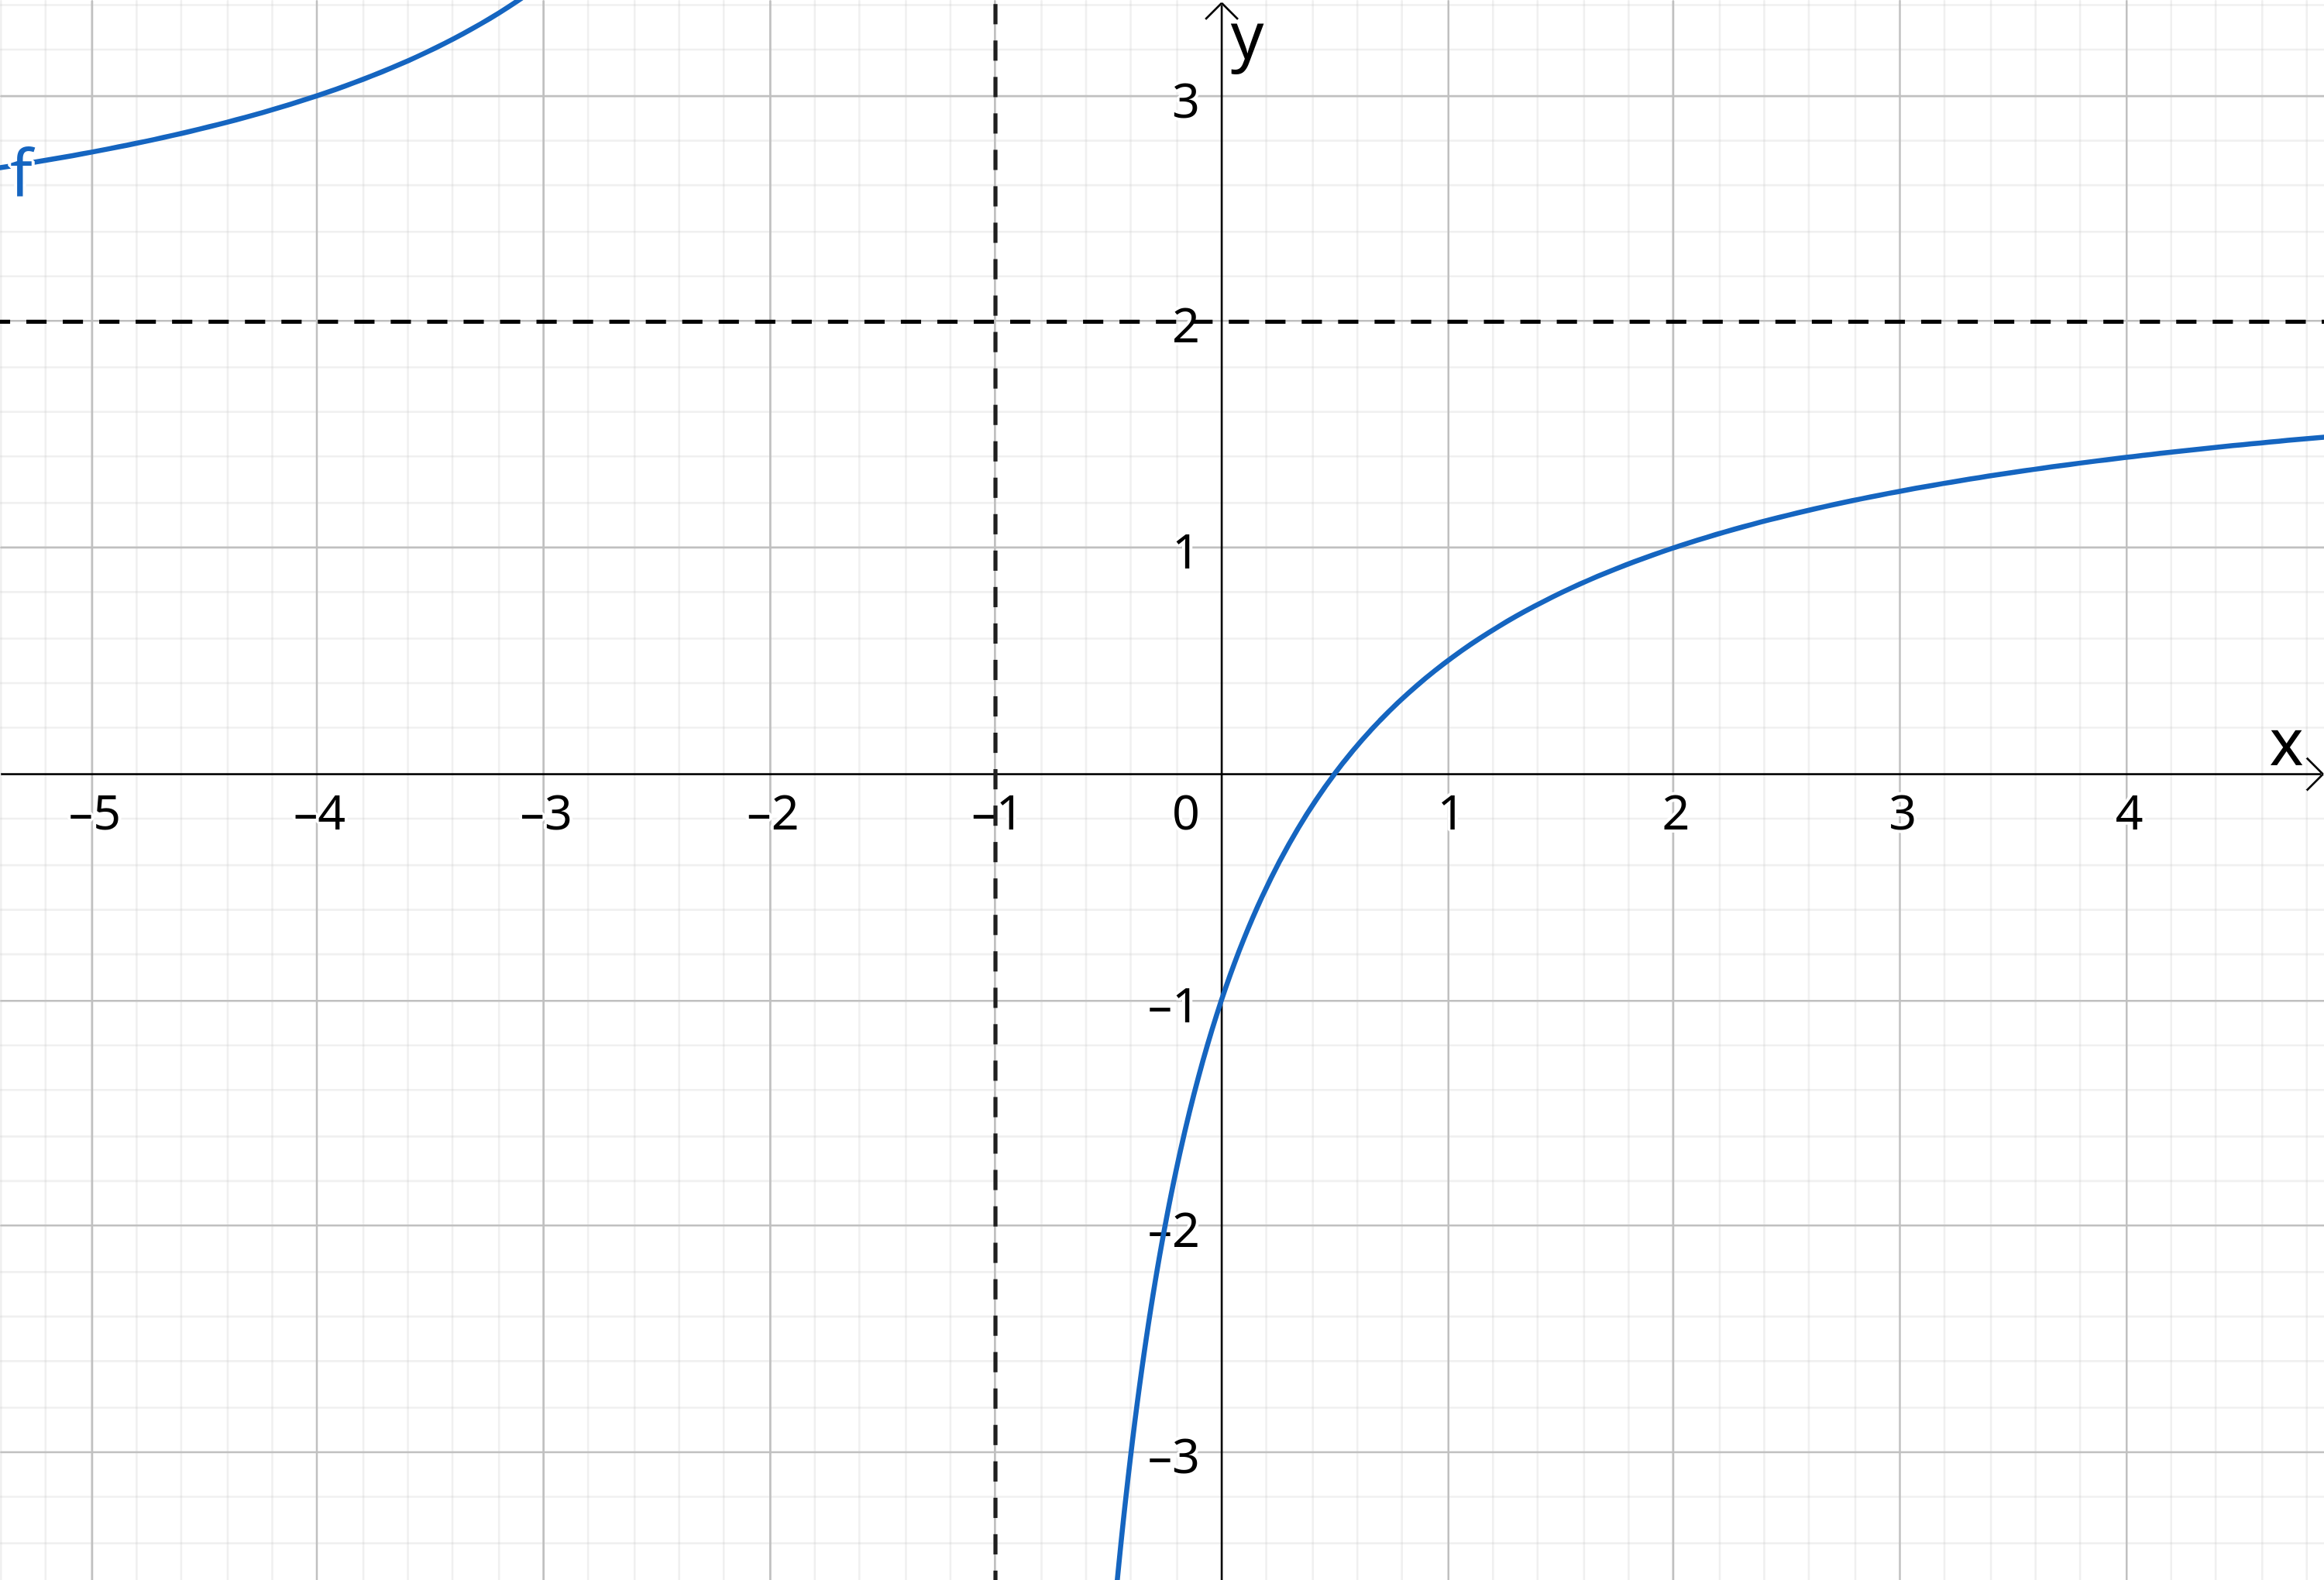
\includegraphics[width=0.5\textwidth]{201001_geogebra-export.png}
\end{center}
%\end{wrapfigure}

    \begin{enumerate}[label={\alph*)}]
         \item Bestimmen Sie $a$ und $b$.
         \item Berechnen Sie die Koordinaten der Schnittpunkte des Pgaphen von $f$ mit demjenigen der linearen Funktion $l:x\rightarrow3x-1$.
         \item Geben Sie eine weitere lineare Funktion an, mit deren Graphen der Graph von $f$ keinen Schnittpunkt besitzt.
         \item Eine Funktion $g$ hat die gleiche Form wie $f$, mit $a=0$ und $b=-2$. Bestimmen Sie die Gleichungen der beiden Asymptoten. Besitzt $g$ eine Nullstelle? Geben Sie diese gegebenfalls an.
         \item Der Funktionsterm der Funktion $h$ ergibt sich aus $h(x)=2x-1+g(x)$. Geben Sie die Gleichungen der Asymptoten von $h$ an.
      \end{enumerate}


\begin{flushright}8BE \end{flushright}

%%%%%%%%%%%%%%%%%%%%%%%%%%%%%%%%%%%%%%%%%%%%%%%%%%%%%%
%%%%%%%%%%%%%%%%%%%%%%%%%%%%%%%%%%%%%%%%%%%%%%%%%%%%%%
\end{document}
